\documentclass[11pt,border=5pt]{standalone}
\usepackage{fontspec}
\setmainfont{cmunrm.otf}[BoldFont=cmunbx.otf,ItalicFont=cmunti.otf,BoldItalicFont=cmunbi.otf]
\usepackage{amsmath}
\usepackage{unicode-math}
\setmathfont{NewCMMath-Regular.otf}
\usepackage{tikz}
\usetikzlibrary{arrows.meta,patterns,angles,quotes}
\begin{document}
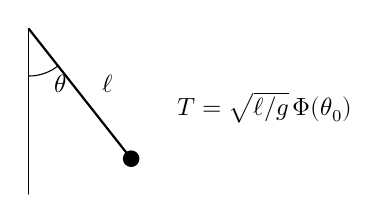
\begin{tikzpicture}[>=Stealth,font=\small,line cap=round,line join=round]
\draw[] (0,0) -- (0,-2.1);
\draw[thick] (0,0) -- (1.3,-1.65);
\fill (1.3,-1.65) circle (3pt);\draw (0,-.6) arc(-90:-52:0.6);\node at (0.4,-0.7) {$\theta$};
\node at (1,-0.7) {$\ell$};
\node at (3,-1) {$T=\sqrt{\ell/g}\,\Phi(\theta_0)$};

\end{tikzpicture}
\end{document}
